\PassOptionsToPackage{usenames,dvipsnames}{xcolor}
\documentclass[xelatex,aspectratio=169]{beamer}

\usepackage{xifthen,multicol,textcomp,graphicx}
\usepackage{fontspec}
\usepackage{tikz,amsmath,xmpp}
\usetikzlibrary{arrows,decorations.pathreplacing}

\usetheme{Atlassian}
\usecolortheme{whale}
\beamertemplatenavigationsymbolsempty

\title[]{XMPP}
\subtitle{Protocol mechanics and common patterns}
\author[]{%
	Sam Whited\\*%
	{\tiny XSF Editor / HipChat Platform Developer}\\*%
	{\tiny JID: \texttt{\href{xmpp:sam@samwhited.com}{sam@samwhited.com}}}%
}
\date{2015--12--18}
\titlegraphic{
\includegraphics[width=20mm]{images/hipchat.png}\hspace*{.25\textwidth}
\includegraphics[width=20mm]{images/atlassian.png}}

% Define a font family that supports IPA characters.
\newfontfamily\ipa{Charis SIL}

\begin{document}

\begin{frame}
	\maketitle
\end{frame}

\begin{frame}
	\ttfamily%
	The following requirements keywords as used in this document are to be
	interpreted as described in RFC 2119: "MUST", "SHALL", "REQUIRED"; "MUST NOT",
	"SHALL NOT"; "SHOULD", "RECOMMENDED"; "SHOULD NOT", "NOT RECOMMENDED"; "MAY",
	"OPTIONAL".
\end{frame}

\begin{frame}
	XMPP is a set of rules for exchanging data between two entities in near-real-time.
\end{frame}

\begin{frame}
	\frametitle{Standards}
	XMPP standardization managed by the IETF. Responsibility for extensions
	delegated to the XMPP Standards Foundation.
	\begin{itemize}
		\item IETF
		\begin{itemize}
			\item \xmppcore\\*(XML-RPC, IoT, RSS/Atom streams, etc.)
			\item \xmppim\ (HipChat!)
			\item \xmppaddr
		\end{itemize}
	\item XSF
		\begin{itemize}
			\item \xep[Multi-User Chat]{0045}
			\item \xep[Stream Management]{0198}
			\item \xep[Entity Versioning]{0366} (yey)
			\item \xep[Message Attaching]{0367} (more yey)
		\item \ldots
		\end{itemize}
	\end{itemize}
\end{frame}

\begin{frame}
	\frametitle{eXtensible Messaging and Presence Protocol}
	\framesubtitle{(from 10,000 feet)}
	\begin{itemize}
		\item XML streams (not documents)
		\item Elements with payloads
			\begin{itemize}
				\item Stanzas: \textit{message, presence, iq}
				\item Nonzas: \textit{auth, compress, \ldots}
			\end{itemize}
		\item Minimal core spec with extensions defined in XEP's
		\item Federated network of servers
	\end{itemize}
\end{frame}

\begin{frame}
\begin{quotation}
	``Extensions are XMPP's greatest strength, and its greatest weakness.''
	\begin{flushright}
		--- Pretty much everyone
	\end{flushright}
\end{quotation}
\end{frame}

\begin{frame}
\begin{center}
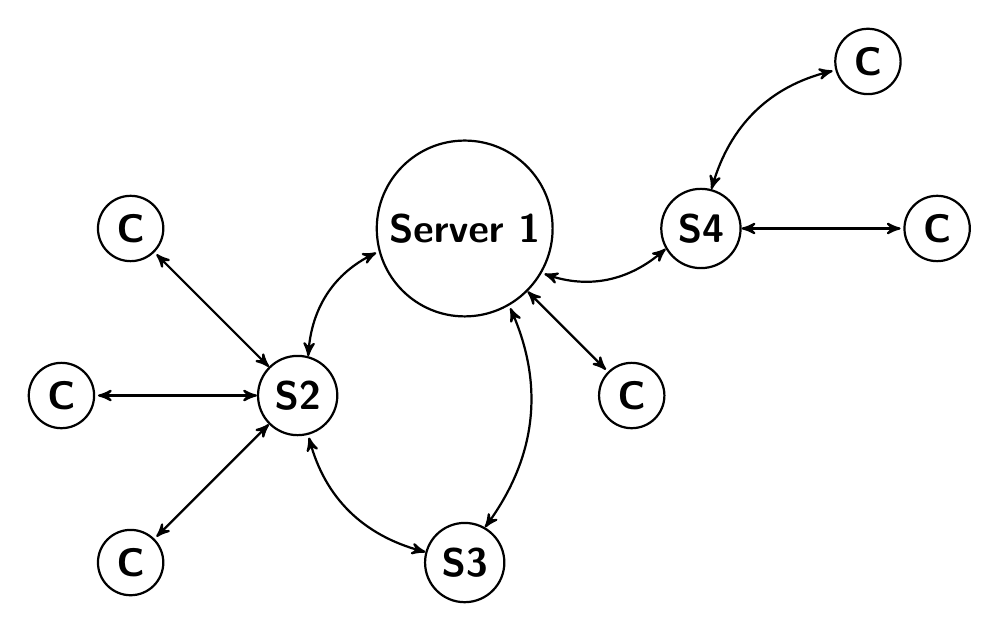
\begin{tikzpicture}[<->,>=stealth',shorten >=1pt,auto,node distance=3cm,
                    thick,main node/.style={circle,draw,font=\sffamily\Large\bfseries}]

  \node[main node] (1) {Server 1};
  \node[main node] (2) [below left of=1] {S2};
  \node[main node] (3) [below right of=2] {S3};
  \node[main node] (4) [right of=1] {S4};

  \node[main node] (5) [above left of=2] {C};
  \node[main node] (6) [      left of=2] {C};
  \node[main node] (7) [below left of=2] {C};
  \node[main node] (8) [right of=4] {C};
  \node[main node] (9) [above right of=4] {C};
  \node[main node] (10) [below right of=1] {C};

  \path[every node/.style={font=\sffamily\small}]
    (1) edge node [right] {} (10)
    (2) edge [bend left] node [right] {} (1)
        edge node [right] {} (5)
        edge node [right] {} (6)
        edge node [right] {} (7)
    (3) edge [bend left] node [right] {} (2)
        edge [bend right] node [right] {} (1)
    (4) edge [bend left] node[right] {} (1)
        edge node [left] {} (8)
        edge [bend left] node [left] {} (9);
\end{tikzpicture}
\end{center}
\end{frame}

\newcommand*{\tikzmark}[1]{\tikz[overlay, remember picture] \coordinate ({#1});}

\begin{frame}
	\frametitle{Anatomy of a JID}
	\Large
	\begin{figure}
		{\color{Navy}%
			\tikzmark{begin}viola\tikzmark{atsep}@%
			\tikzmark{domainpart}shakespeare.lit\tikzmark{slashsep}/%
			\tikzmark{resourcepart}ilyria\tikzmark{end}%
		}

		\tikz[overlay,remember picture] {
			\draw[decorate,decoration={brace,raise=5mm,amplitude=20pt}] (begin.north west) -- node [above=2.5em] {JID} (end.north east) ;
			\draw[decorate,decoration={brace,raise=2mm,amplitude=5pt,mirror}] (begin.south west) -- node[below of=begin, below=-1.25em] {\small localpart} (atsep.south west) ;
			\draw[decorate,decoration={brace,raise=2mm,amplitude=10pt,mirror}] (domainpart.south west) -- node[below of=begin, below=-1em] {\small domainpart} (slashsep.south west) ;
			\draw[decorate,decoration={brace,raise=2mm,amplitude=5pt,mirror}] (resourcepart.south east) -- node[below of=begin, below=-1.25em] {\small resourcepart} (end.south east) ;
		}
	\end{figure}
\end{frame}
\begin{frame}
	\frametitle{Anatomy of a JID}
	\Large
	\begin{figure}
		\tikzmark{begin}\textcolor{Violet}{viola}\tikzmark{atsep}@%
		\tikzmark{domainpart}shakespeare.lit\tikzmark{slashsep}/%
		\tikzmark{resourcepart}ilyria\tikzmark{end}%

		\tikz[overlay,remember picture] {
			\draw[decorate,decoration={brace,raise=5mm,amplitude=20pt}] (begin.north west) -- node [above=2.5em] {JID} (end.north east) ;
			\draw[decorate,decoration={brace,raise=2mm,amplitude=5pt,mirror}] (begin.south west) -- node[below of=begin, below=-1.25em] {\small localpart} (atsep.south west) ;
			\draw[decorate,decoration={brace,raise=2mm,amplitude=10pt,mirror}] (domainpart.south west) -- node[below of=begin, below=-1em] {\tiny domainpart} (slashsep.south west) ;
			\draw[decorate,decoration={brace,raise=2mm,amplitude=5pt,mirror}] (resourcepart.south east) -- node[below of=begin, below=-1.25em] {\tiny resourcepart} (end.south east) ;
		}
	\end{figure}
\end{frame}
\begin{frame}
	\frametitle{Anatomy of a JID}
	\Large
	\begin{figure}
		\tikzmark{begin}viola\tikzmark{atsep}@%
		\tikzmark{domainpart}\textcolor{LimeGreen}{shakespeare.lit}\tikzmark{slashsep}/%
		\tikzmark{resourcepart}ilyria\tikzmark{end}

		\tikz[overlay,remember picture] {
			\draw[decorate,decoration={brace,raise=5mm,amplitude=20pt}] (begin.north west) -- node [above=2.5em] {JID} (end.north east) ;
			\draw[decorate,decoration={brace,raise=2mm,amplitude=5pt,mirror}] (begin.south west) -- node[below of=begin, below=-1.25em] {\tiny localpart} (atsep.south west) ;
			\draw[decorate,decoration={brace,raise=2mm,amplitude=10pt,mirror}] (domainpart.south west) -- node[below of=begin, below=-1em] {\small domainpart} (slashsep.south west) ;
			\draw[decorate,decoration={brace,raise=2mm,amplitude=5pt,mirror}] (resourcepart.south east) -- node[below of=begin, below=-1.25em] {\tiny resourcepart} (end.south east) ;
		}
	\end{figure}
\end{frame}
\begin{frame}
	\frametitle{Anatomy of a JID}
	\Large
	\begin{figure}
		\tikzmark{begin}viola\tikzmark{atsep}@%
		\tikzmark{domainpart}shakespeare.lit\tikzmark{slashsep}/%
		\tikzmark{resourcepart}\textcolor{CheetoOrange}{ilyria}\tikzmark{end}

		\tikz[overlay,remember picture] {
			\draw[decorate,decoration={brace,raise=5mm,amplitude=20pt}] (begin.north west) -- node [above=2.5em] {JID} (end.north east) ;
			\draw[decorate,decoration={brace,raise=2mm,amplitude=5pt,mirror}] (begin.south west) -- node[below of=begin, below=-1.25em] {\tiny localpart} (atsep.south west) ;
			\draw[decorate,decoration={brace,raise=2mm,amplitude=10pt,mirror}] (domainpart.south west) -- node[below of=begin, below=-1em] {\tiny domainpart} (slashsep.south west) ;
			\draw[decorate,decoration={brace,raise=2mm,amplitude=5pt,mirror}] (resourcepart.south east) -- node[below of=begin, below=-1.25em] {\small resourcepart} (end.south east) ;
		}
	\end{figure}
\end{frame}

\section[]{XMPP Core}
\frame{\sectionpage}

\begin{frame}
	\frametitle{Stream's}
	\begin{itemize}
		\item Client first
		\item Two streams (input and output)
		\item Streams are restarted when their state changes (eg. TLS or stream
			compression is started, feature negotiation happens, etc.)
		\item Event based and pipelined (async communication)
	\end{itemize}
\end{frame}

\subsection[]{Stream Initialization and Feature Negotiation}
\frame{\subsectionpage}

\begin{frame}
	\begin{multicols}{2}
		\begin{flushleft}
			\centerline{Client}
		\end{flushleft}
		\columnbreak
		\begin{flushleft}
			\centerline{Server}
		\end{flushleft}
	\end{multicols}
\end{frame}
\begin{frame}
	\begin{multicols}{2}
		\begin{flushleft}
			\centerline{Client}
			\procinst\\
			\xml{stream:stream \ldots}
		\end{flushleft}
		\columnbreak
		\begin{flushleft}
			\centerline{Server}
		\end{flushleft}
	\end{multicols}
\end{frame}
\begin{frame}
	\begin{multicols}{2}
		\begin{flushleft}
			\centerline{Client}
			\procinst\\
			\xml{stream:stream \ldots}
		\end{flushleft}
		\columnbreak
		\begin{flushleft}
			\centerline{Server}
			\vspace{2em}
			\procinst\\
			\xml{stream:stream \ldots}
		\end{flushleft}
	\end{multicols}
\end{frame}
\begin{frame}
	\begin{multicols}{2}
		\begin{flushleft}
			\centerline{Client}
			\procinst\\
			\xml{stream:stream \ldots}
		\end{flushleft}
		\columnbreak
		\begin{flushleft}
			\centerline{Server}
			\vspace{2em}
			\procinst\\
			\xml{stream:stream \ldots}\\
			\xml{stream:features}\\
			\xml{starttls \ldots}\\
			\xml{required /}\\
			\xml*{starttls}\\
			\xml*{stream:features}
		\end{flushleft}
	\end{multicols}
\end{frame}
\begin{frame}
	\begin{multicols}{2}
		\begin{flushleft}
			\centerline{Client}
			\procinst\\
			\xml{stream:stream \ldots}\\
			\vspace*{8em}
			\xml{starttls \ldots /}
		\end{flushleft}
		\columnbreak
		\begin{flushleft}
			\centerline{Server}
			\vspace{2em}
			\procinst\\
			\xml{stream:stream \ldots}\\
			\xml{stream:features}\\
			\xml{starttls \ldots}\\
			\xml{required /}\\
			\xml*{starttls}\\
			\xml*{stream:features}
		\end{flushleft}
	\end{multicols}
\end{frame}
\begin{frame}
	\begin{multicols}{2}
		\begin{flushleft}
			\centerline{Client}
			\procinst\\
			\xml{stream:stream \ldots}\\
			\vspace*{8em}
			\xml{starttls \ldots /}
		\end{flushleft}
		\columnbreak
		\begin{flushleft}
			\centerline{Server}
			\vspace{2em}
			\procinst\\
			\xml{stream:stream \ldots}\\
			\xml{stream:features}\\
			\xml{starttls \ldots}\\
			\xml{required /}\\
			\xml*{starttls}\\
			\xml*{stream:features}\\
			\vspace*{1em}
			\xml{proceed \ldots /}
		\end{flushleft}
	\end{multicols}
\end{frame}
\begin{frame}
	\begin{multicols}{2}
		\begin{flushleft}
			\centerline{Client}
			\procinst\\
			\xml{stream:stream \ldots}\\
			\vspace*{8em}
			\xml{starttls \ldots /}\\
			\ \\
			01000111011001010111010000100000011000100110000101100011011010110010\\
			00000111010001101111001000000111011101101111011100100110101100101110
		\end{flushleft}
		\columnbreak
		\begin{flushleft}
			\centerline{Server}
			\vspace*{2em}
			\procinst\\
			\xml{stream:stream \ldots}\\
			\xml{stream:features}\\
			\xml{starttls \ldots}\\
			\xml{required /}\\
			\xml*{starttls}\\
			\xml*{stream:features}\\
			\vspace*{1em}
			\xml{proceed \ldots /}\\
		\end{flushleft}
	\end{multicols}
\end{frame}
\begin{frame}
	\begin{multicols}{2}
		\begin{flushleft}
			\centerline{Client}
			\procinst\\
			\xml{stream:stream \ldots}\\
			\vspace*{8em}
			\xml{starttls \ldots /}\\
			\ \\
			01000111011001010111010000100000011000100110000101100011011010110010\\
			00000111010001101111001000000111011101101111011100100110101100101110
			\xml{stream:stream \ldots}
		\end{flushleft}
		\columnbreak
		\begin{flushleft}
			\centerline{Server}
			\vspace*{2em}
			\procinst\\
			\xml{stream:stream \ldots}\\
			\xml{stream:features}\\
			\xml{starttls \ldots}\\
			\xml{required /}\\
			\xml*{starttls}\\
			\xml*{stream:features}\\
			\vspace*{1em}
			\xml{proceed \ldots /}\\
		\end{flushleft}
	\end{multicols}
\end{frame}
\begin{frame}
	\begin{multicols}{2}
		\begin{flushleft}
			\centerline{Client}
			\procinst\\
			\xml{stream:stream \ldots}\\
			\vspace*{8em}
			\xml{starttls \ldots /}\\
			\ \\
			01000111011001010111010000100000011000100110000101100011011010110010\\
			00000111010001101111001000000111011101101111011100100110101100101110
			\xml{stream:stream \ldots}
		\end{flushleft}
		\columnbreak
		\begin{flushleft}
			\centerline{Server}
			\vspace*{2em}
			\procinst\\
			\xml{stream:stream \ldots}\\
			\xml{stream:features}\\
			\xml{starttls \ldots}\\
			\xml{required /}\\
			\xml*{starttls}\\
			\xml*{stream:features}\\
			\vspace*{1em}
			\xml{proceed \ldots /}\\
			\vspace*{4em}
			\xml{stream:stream \ldots}
		\end{flushleft}
	\end{multicols}
\end{frame}
{
\begin{frame}
	\begin{multicols}{2}
		\begin{flushleft}
			\centerline{Client}
			\vspace*{5em}
			\xml{starttls \ldots /}\\
			\vspace*{2em}
			01000111011001010111010000100000011000100110000101100011011010110010\\
			00000111010001101111001000000111011101101111011100100110101100101110
			\xml{stream:stream \ldots}
		\end{flushleft}
		\columnbreak
		\begin{flushleft}
			\centerline{Server}
			\xml{starttls \ldots}\\
			\xml{required /}\\
			\xml*{starttls}\\
			\xml*{stream:features}\\
			\vspace*{1em}
			\xml{proceed \ldots /}\\
			\vspace*{5em}
			\xml{stream:stream \ldots}\\
			\xml{stream:features \ldots}\\
			\xml{mechanisms \ldots}\\
			\xml{mechanism}\texttt{SCRAM-SHA-1}\xml*{mechanism}
			\xml*{mechanisms}\\
		\end{flushleft}
	\end{multicols}
\end{frame}
\begin{frame}
	\begin{multicols}{2}
		\begin{flushleft}
			\centerline{Client}
			\vspace*{4em}
			\xml{starttls \ldots /}\\
			\vspace*{2em}
			01000111011001010111010000100000011000100110000101100011011010110010\\
			00000111010001101111001000000111011101101111011100100110101100101110
			\xml{stream:stream \ldots}\\
			\vspace*{6em}
			\xml{auth}
		\end{flushleft}
		\columnbreak
		\begin{flushleft}
			\centerline{Server}
			\xml{required /}\\
			\xml*{starttls}\\
			\xml*{stream:features}\\
			\vspace*{1em}
			\xml{proceed \ldots /}\\
			\vspace*{5em}
			\xml{stream:stream \ldots}\\
			\xml{stream:features \ldots}\\
			\xml{mechanisms \ldots}\\
			\xml{mechanism}\texttt{SCRAM-SHA-1}\xml*{mechanism}
			\xml*{mechanisms}\\
		\end{flushleft}
	\end{multicols}
\end{frame}
\begin{frame}
	\begin{multicols}{2}
		\begin{flushleft}
			\centerline{Client}
			\vspace*{3em}
			\xml{starttls \ldots /}\\
			\vspace*{2em}
			01000111011001010111010000100000011000100110000101100011011010110010\\
			00000111010001101111001000000111011101101111011100100110101100101110
			\xml{stream:stream \ldots}\\
			\vspace*{5em}
			\xml{auth}\\
			\ldots
		\end{flushleft}
		\columnbreak
		\begin{flushleft}
			\centerline{Server}
			\xml*{starttls}\\
			\xml*{stream:features}\\
			\vspace*{1em}
			\xml{proceed \ldots /}\\
			\vspace*{5em}
			\xml{stream:stream \ldots}\\
			\xml{stream:features \ldots}\\
			\xml{mechanisms \ldots}\\
			\xml{mechanism}\texttt{SCRAM-SHA-1}\xml*{mechanism}
			\xml*{mechanisms}\\
		\end{flushleft}
	\end{multicols}
\end{frame}
\begin{frame}
	\begin{multicols}{2}
		\begin{flushleft}
			\centerline{Client}
			\vspace*{2em}
			\xml{starttls \ldots /}\\
			\vspace*{2em}
			01000111011001010111010000100000011000100110000101100011011010110010\\
			00000111010001101111001000000111011101101111011100100110101100101110
			\xml{stream:stream \ldots}\\
			\vspace*{5em}
			\xml{auth}\\
			\ldots\\
			\ldots
		\end{flushleft}
		\columnbreak
		\begin{flushleft}
			\centerline{Server}
			\xml*{stream:features}\\
			\vspace*{1em}
			\xml{proceed \ldots /}\\
			\vspace*{5em}
			\xml{stream:stream \ldots}\\
			\xml{stream:features \ldots}\\
			\xml{mechanisms \ldots}\\
			\xml{mechanism}\texttt{SCRAM-SHA-1}\xml*{mechanism}
			\xml*{mechanisms}\\
		\end{flushleft}
	\end{multicols}
\end{frame}
\begin{frame}
	\begin{multicols}{2}
		\begin{flushleft}
			\centerline{Client}
			\vspace*{1em}
			\xml{starttls \ldots /}\\
			\vspace*{2em}
			01000111011001010111010000100000011000100110000101100011011010110010\\
			00000111010001101111001000000111011101101111011100100110101100101110
			\xml{stream:stream \ldots}\\
			\vspace*{5em}
			\xml{auth}\\
			\ldots\\
			\ldots\\
			\ldots
		\end{flushleft}
		\columnbreak
		\begin{flushleft}
			\centerline{Server}
			\vspace*{1em}
			\xml{proceed \ldots /}\\
			\vspace*{5em}
			\xml{stream:stream \ldots}\\
			\xml{stream:features \ldots}\\
			\xml{mechanisms \ldots}\\
			\xml{mechanism}\texttt{SCRAM-SHA-1}\xml*{mechanism}
			\xml*{mechanisms}\\
		\end{flushleft}
	\end{multicols}
\end{frame}
}

\begin{frame}
	\vspace*{\fill}
	
\includegraphics[width=.75\textwidth]{images/deeper.jpg}
\end{frame}

\subsection[]{Inside the stream}
\begin{frame}
\subsectionpage
\centerline{(post resource binding)}
\end{frame}

\begin{frame}
\vspace*{\fill}
\textbf{Stanza} \ipa{/ˈstænzə/} (\kern1pt\textit{plural} stanzas) n.
\begin{enumerate}
	\item A unit of a poem, written or printed as a paragraph; equivalent to a verse.
	\item (computing) An XML element which acts as basic unit of meaning in XMPP.
\end{enumerate}
\vspace*{\fill}
\end{frame}

\begin{frame}
	\frametitle{Stanza's}
	The basic primitives of XMPP.
	\begin{itemize}
		\item \stanza{message}
		\item \stanza{iq}
		\item \stanza{presence}
	\end{itemize}

	Generally speaking, these should be the only things sent at the top level of
	an XMPP stream (with a few exceptions, eg. \xep{0198} keep-alive's).
\end{frame}

\begin{frame}[fragile]
	\frametitle{\stanza{message}}
	\begin{itemize}
	\item One-to-one
	\item Fire and forget
	\item No delivery guarantee (ack)
	\item Useful for anything that does not require a response (chats, alerts, log lines, etc.)
	\end{itemize}
	\begin{lstlisting}[frame=single,language=xml]
<message id='262' type='chat'
  to='feste@shakespeare.lit/house'>
  <body>
    What&apos;s a drunken man like, fool?
  </body>
  <request xmlns='urn:xmpp:receipts'/>
  <thread>pNltztLMBQhqakHwcFd</thread>
</message>
\end{lstlisting}
\end{frame}

\begin{frame}[fragile]
	\frametitle{\stanza{iq} (``Information query'')}
		\begin{itemize}
		\item One-to-one
		\item MUST send a response
		\item At-least-once delivery (cache and resend if no result)
		\end{itemize}
\begin{lstlisting}[frame=single,language=xml]
<iq from='capulet.lit'
  to='juliet@capulet.lit/balcony'
  id='s2c1' type='get'>
  <ping xmlns='urn:xmpp:ping'/>
</iq>

<iq to='capulet.lit'
  from='juliet@capulet.lit/balcony'
  id='s2c1' type='result'/>
\end{lstlisting}
\end{frame}

\begin{frame}[fragile]
	\frametitle{\stanza{presence}}
	\begin{itemize}
	\item Directed (one-to-one) or broadcast (one-to-many)
	\item Advertises entity availability to the network
	\item Payload's for broadcast can ride along (entity capabilities, status
		messages, etc.)
	\end{itemize}
\begin{lstlisting}[frame=single,language=xml]
<presence id='24'
  from='prospero@shakespeare.lit/cell'>
  <status>
    Now my charms are all o&apos;erthrown
  </status>
  <priority>40</priority>
  <show>away</show>
</presence>
\end{lstlisting}
\end{frame}

\begin{frame}
	\frametitle{Stanza Types}
	Stanza's (and some nonza's) MAY have a `type' attribute. For messages, the
	type conveys semantic meaning and is non-normative. For IQ's, the type is much
	more strictly controlled.
	\begin{multicols}{2}
		Message types
	\begin{itemize}
		\item\textit{normal}
		\item\textit{chat}
		\item\textit{groupchat}
		\item\textit{headline}
		\item\textit{error}
	\end{itemize}
	\columnbreak
	IQ types
	\begin{itemize}
		\item\textit{get}
		\item\textit{set}
		\item\textit{result}
		\item\textit{error}
	\end{itemize}
	\end{multicols}
\end{frame}

\begin{frame}
\begin{quotation}
``XMPP is Sacred''
\begin{flushright}
---\xep[XMPP Design Guidelines]{0134}
\end{flushright}
\vspace*{2em}
When designing a new extension, think very hard about your life before you
invent new stream level elements, and never modify core protocol.
\end{quotation}
\end{frame}

\begin{frame}[fragile]
	\frametitle{Namespacing}
	\begin{flushleft}
		Stanza payloads are handled based on their XML namespace. By recent
		convention, namespaces are versioned URN's.
	\end{flushleft}
\begin{lstlisting}[frame=single,language=xml]
<message from='juliet@capulet.lit'
         to='romeo@montague.lit/orchard'
         type='headline' id='tfasd'>
  <result xmlns='urn:xmpp:mam:1' queryid='f27'
          id='5d398-28273-f7382'>
  ...
  </result>
</message>
\end{lstlisting}
\end{frame}

\section[]{Useful Extensions}
\frame{\sectionpage}

\begin{frame}
	\frametitle{\xep[Message Carbons]{0280}}
	\begin{itemize}
		\item Copies incoming messages to resources that would otherwise not have received the message.
		\item Copies outgoing messages to your other connected resources
		\item Current behavior not well defined for special messages (Typing notifications, read state markers, etc.)
		\item It's simple and gets the job done
		\item One day might be replaced by\ldots
	\end{itemize}
\end{frame}

\begin{frame}
	\frametitle{\xep[Message Archive Management (MAM)]{0313}}
	\begin{itemize}
		\item Stores incoming and outgoing messages on server
		\item New clients can access history
		\item Clients that have been offline can catch up
		\item Currently relies on synchronized clocks between client and server (facepalm)
		\item Work is being done to make it possible to query the archive for
			messages after a given ID.
	\end{itemize}
\end{frame}

\begin{frame}
	\frametitle{Myth № 1: XMPP is bad on mobile}
	Turns out that XMPP is actually \emph{very} good on mobile devices, both on
	battery and bandwidth. Historically, mobile \emph{clients} have been very bad.
\end{frame}

\begin{frame}[fragile]
	\frametitle{\xep[Client State Indication (CSI)]{0352}}
	Clients indicate when they become ``inactive'' (screen goes off, app loses
	focus, etc.) or ``active'' with some simple nonza's. Server does what it wants
	with that data (eg. don't send presence or typing notifications and start
	sending push notifications).
	\vspace*{\fill}
\begin{lstlisting}[frame=single,language=xml]
<active xmlns='urn:xmpp:csi:0'/>
<inactive xmlns='urn:xmpp:csi:0'/>
\end{lstlisting}
\vspace*{\fill}
\end{frame}

\begin{frame}
	\frametitle{\xep[Mobile Considerations]{0268}}
	\begin{flushleft}
		Attempts to tell you everything you need to know about not eating your users'
		battery (with citations).
	\end{flushleft}
	\begin{flushleft}
		TL;DR --- Implement CSI, and when you detect that something is already being
		sent/received: Send/receive as much data as you can at once so the radio can
		go back to sleep. Compression is also good.
	\end{flushleft}
	\begin{flushleft}
		Disclaimer: I wrote this one and don't do much mobile development. It's
		probably all wrong (but seems to be working out so far).
	\end{flushleft}
\end{frame}

\begin{frame}
	\frametitle{\xep[Stream Management]{0198}}
	\begin{itemize}
		\item Stream resumption (very fast reconnects)
		\item Stanza acknowledgements
	\end{itemize}

	Has some problems around ``zombie state's'' where clients are offline, but the
	stream hasn't timed out yet. Like most things, the answer is probably MAM.
\end{frame}

\newfontfamily\calluna{Calluna}
\begin{frame}
	\Large
	\calluna
	\begin{figure}
	{\color{AshGray}%
		\tikzmark{begin}sam\tikzmark{atsep}@%
		\tikzmark{domainpart}\textcolor{Cyan}{SamWhited}\tikzmark{tld}.com\tikzmark{end}%
	}

		\tikz[overlay,remember picture] {
			\draw[decorate,decoration={brace,raise=5mm,amplitude=15pt}] (begin.north
			west) -- node [above=1.75em] {\small email \& jid} (end.north east) ;
			\draw[decorate,decoration={brace,raise=2mm,amplitude=5pt,mirror}]
			(begin.south west) -- node[below of=begin, below=-1.35em] {\tiny me} (atsep.south west) ;
			\draw[decorate,decoration={brace,raise=2mm,amplitude=5pt,mirror}]
			(atsep.south west) -- node[below of=begin, below=-1.35em] {\tiny twitter
			\addfontfeature{Variant=1}{\&} hipchat } (tld.south west) ;
			\draw[decorate,decoration={brace,raise=6mm,amplitude=10pt,mirror}]
			(domainpart.south west) -- node[below of=begin, below=-.125em] {\tiny blog} (end.south west) ;
		}
	\end{figure}
\end{frame}

\end{document}
